\documentclass[preprint,12pt,authoryear]{elsarticle}

\usepackage[T1]{fontenc}
\usepackage[utf8]{inputenc}
\usepackage{lmodern}
\usepackage{amsmath,amssymb,bm,mathtools}
\usepackage{booktabs,tabularx,longtable,array,multirow}
\usepackage{graphicx,subcaption,float}
\usepackage{siunitx}
\usepackage{xcolor}
\usepackage{microtype}
\usepackage{enumitem}
\usepackage{url}
\usepackage{hyperref}
\usepackage[nameinlink,capitalize,noabbrev]{cleveref}

\graphicspath{{figures/}}
\setlength{\emergencystretch}{3em}
% Shared mathematical notation.
\newcommand{\Y}{\mathbf{Y}}
\newcommand{\X}{\mathbf{X}}
\newcommand{\calX}{\mathcal{X}}
\newcommand{\E}{\mathbb{E}}
\newcommand{\Var}{\operatorname{Var}}
\newcommand{\Cov}{\operatorname{Cov}}
\newcommand{\Corr}{\operatorname{Corr}}
\newcommand{\median}{\operatorname{median}}
\newcommand{\MAD}{\operatorname{MAD}}
\newcommand{\argmax}{\operatorname*{arg\,max}}
\newcommand{\ROI}{\mathrm{ROI}}
\newcommand{\SNR}{\mathrm{SNR}}
\newcommand{\LOBO}{\mathrm{LOBO}}
\newcommand{\LOSO}{\mathrm{LOSO}}
\newcommand{\PU}{\mathrm{PU}}
\newcommand{\dd}{\,\mathrm{d}}

% Draft and provisional-result helpers.
\definecolor{provisionalorange}{RGB}{166,82,0}
\definecolor{draftred}{RGB}{155,25,25}
\newif\ifshowprovisional
\showprovisionaltrue

\newcommand{\Provisional}[1]{%
  \ifshowprovisional
    \textcolor{provisionalorange}{#1}\textsuperscript{\textcolor{provisionalorange}{\ensuremath{\dagger}}}%
  \else
    #1%
  \fi
}
\newcommand{\Missing}[1]{\textcolor{draftred}{[MISSING: #1]}}
\newcommand{\AuthorDecision}[1]{\textcolor{draftred}{[AUTHOR DECISION: #1]}}
\newcommand{\CodexReplace}[1]{\textcolor{draftred}{[CODEX REPLACE: #1]}}
\newcommand{\DraftOnly}[1]{\textcolor{draftred}{#1}}
\newcommand{\DraftBanner}{%
  \begin{center}
  \fcolorbox{draftred}{red!3}{%
  \parbox{0.93\linewidth}{\small\textbf{Complete working manuscript; author review required.}
  Daggered values remain explicitly provisional and are excluded from the main claim path.
  Author, ethics, funding, data-release, and final adjudication fields require review.
  The release build must disable provisional mode and contain no red placeholders.}}
  \end{center}
}

\newcommand{\DraftFigure}[3]{%
\begin{figure}[!htbp]
  \centering
  \fbox{\parbox[c][0.23\textheight][c]{0.90\linewidth}{\centering
  \textbf{Planned figure}\par\medskip #1}}
  \caption{#2}
  \label{#3}
\end{figure}}

\newcommand{\ProvisionalFigure}[4]{%
\begin{figure}[!htbp]
  \centering
  \IfFileExists{figures/#2}{\includegraphics[width=#1]{#2}}{%
    \fbox{\parbox[c][0.20\textheight][c]{0.90\linewidth}{\centering Missing provisional asset: \nolinkurl{#2}}}}
  \caption{#3 \textbf{Provisional:} this artifact predates the identity/geometry repair and is included only to guide the confirmatory rerun.}
  \label{#4}
\end{figure}}

% Generated by scripts/build_results_macros.py; do not edit by hand.
\newcommand{\ResultsGeneratedOn}{2026-08-24}
\newcommand{\ResultsSourceStatus}{pre-repair repository audit}

\newcommand{\CarrierRecallBtwenty}{\Provisional{\ensuremath{0.5409}}}
\newcommand{\CertaintyDominantClassCramersV}{\ensuremath{0.346}}
\newcommand{\CertaintyDominantClassPermutationP}{\ensuremath{0.313}}
\newcommand{\CoherenceRecallBtwenty}{\Provisional{\ensuremath{0.6053}}}
\newcommand{\ICADiffRSquared}{\Provisional{\ensuremath{0.9938}}}
\newcommand{\ICADiffScoreCorrelation}{\Provisional{\ensuremath{0.9988}}}
\newcommand{\ICADiffShiftP}{\Provisional{\ensuremath{0.005}}}
\newcommand{\LagRecallBtwenty}{\Provisional{\ensuremath{0.6220}}}
\newcommand{\LeftRightGlobalCorrelation}{\Provisional{\ensuremath{0.557}}}
\newcommand{\NCurrentBursts}{\Provisional{4}}
\newcommand{\NCurrentCanonicalNeurons}{\Provisional{26}}
\newcommand{\NCurrentOccurrences}{\Provisional{79}}
\newcommand{\NCurrentOriginalSites}{\Provisional{27}}
\newcommand{\NCurrentRecordings}{\Provisional{1}}
\newcommand{\ProvisionalFieldBoundaryX}{\Provisional{\ensuremath{x=286}}}
\newcommand{\QuietVarianceSlope}{\Provisional{\ensuremath{3.63}}}
\newcommand{\QuietVarianceWeightedRtwo}{\Provisional{\ensuremath{0.955\text{--}0.959}}}
\newcommand{\RawAnnulusCIHigh}{\Provisional{\ensuremath{0.0008}}}
\newcommand{\RawAnnulusCILow}{\Provisional{\ensuremath{-0.0277}}}
\newcommand{\RawAnnulusDelta}{\Provisional{\ensuremath{-0.0131}}}
\newcommand{\RawFirstPCVariance}{\Provisional{\ensuremath{87.4\%}}}
\newcommand{\RawHeldoutCorrelation}{\Provisional{\ensuremath{0.8256}}}
\newcommand{\RawWithinSiteMedianCorrelation}{\Provisional{\ensuremath{0.3720}}}
\newcommand{\ResidualHeldoutCorrelation}{\Provisional{\ensuremath{0.5307}}}
\newcommand{\ResidualPeakAmplitudeCIHigh}{\Provisional{\ensuremath{140.75}}}
\newcommand{\ResidualPeakAmplitudeCILow}{\Provisional{\ensuremath{50.64}}}
\newcommand{\ResidualPeakAmplitudeDelta}{\Provisional{\ensuremath{91.33}}}
\newcommand{\ResidualSpatialCIHigh}{\Provisional{\ensuremath{0.0472}}}
\newcommand{\ResidualSpatialCILow}{\Provisional{\ensuremath{-0.2560}}}
\newcommand{\ResidualSpatialDelta}{\Provisional{\ensuremath{-0.0953}}}
\newcommand{\ResidualWithinSiteMedianCorrelation}{\Provisional{\ensuremath{0.3144}}}
\newcommand{\SpatialICAContrastDelta}{\ensuremath{0.170}}
\newcommand{\SpatialICAContrastQ}{\ensuremath{0.0001}}
\newcommand{\SpatialICAMinEventMapCorrelation}{\ensuremath{0.9983}}
\newcommand{\SpatialICAMinMorphologySpearman}{\ensuremath{0.9948}}
\newcommand{\SpatialICAMinPixelCorrelation}{\ensuremath{0.9985}}
\newcommand{\SpatialICAPeakOffsetDelta}{\ensuremath{-3.990}}
\newcommand{\SpatialICAPeakOffsetQ}{\ensuremath{0.0003}}
\newcommand{\SpatialICARadiusDelta}{\ensuremath{-1.335}}
\newcommand{\SpatialICARadiusQ}{\ensuremath{0.0014}}
\newcommand{\SpatialICAReferenceRecall}{\ensuremath{0.6714}}
\newcommand{\SpatialICAVsevenBoundaryEpsilon}{\ensuremath{0.323}}
\newcommand{\SpatialICAVsevenBoundaryQ}{\ensuremath{0.0679}}

% Generated by scripts/import_fig08_full_trace_feature_panel.py; do not edit.
\newcommand{\FullTraceOccurrences}{106}
\newcommand{\FullTraceSites}{50}
\newcommand{\FullTraceCarrierPercentile}{0.994}
\newcommand{\FullTraceCarrierCILow}{0.981}
\newcommand{\FullTraceCarrierCIHigh}{1.000}
\newcommand{\FullTraceCoherencePercentile}{0.994}
\newcommand{\FullTraceLagPercentile}{0.996}
\newcommand{\FullTraceLagDelta}{+0.002}
\newcommand{\FullTraceLagDeltaLow}{0.000}
\newcommand{\FullTraceLagDeltaHigh}{0.006}
\newcommand{\FullTraceRawPercentile}{0.991}
\newcommand{\FullTraceConsensusPercentile}{0.986}
\newcommand{\FullTraceConsensusRepeatability}{0.633}
\newcommand{\FullTracePersistencePercentile}{0.972}
\newcommand{\FullTracePersistenceRepeatability}{0.649}
\newcommand{\FullTraceVSTPercentile}{0.883}
\newcommand{\FullTraceCarrierCeilingCount}{104}
\newcommand{\FullTraceCoherenceCeilingCount}{104}
\newcommand{\FullTraceLagCeilingCount}{105}

% Generated by scripts/import_fig09_automated_feature_validation.py; do not edit.
\newcommand{\AutoRawAUC}{0.931}
\newcommand{\AutoRawAUCLow}{0.906}
\newcommand{\AutoRawAUCHigh}{0.952}
\newcommand{\AutoCarrierAUC}{0.920}
\newcommand{\AutoCoherenceAUC}{0.915}
\newcommand{\AutoLagAUC}{0.905}
\newcommand{\AutoMatchedAUC}{0.884}
\newcommand{\AutoPersistenceSpatialDelta}{0.217}
\newcommand{\AutoRecoveryCount}{94}
\newcommand{\AutoRecoveryMisses}{12}
\newcommand{\AutoCarrierLogLoss}{0.712}
\newcommand{\AutoExtendedLogLoss}{0.577}
\newcommand{\AutoRecoveryDelta}{0.136}
\newcommand{\AutoRecoveryDeltaLow}{-0.025}
\newcommand{\AutoRecoveryDeltaHigh}{0.280}
\newcommand{\AutoCarrierReliability}{0.580}
\newcommand{\AutoAnnulusReliability}{0.866}
\newcommand{\AutoNullP}{0.0020}

% Generated by scripts/import_fig11_feature_deep_dives.py; do not edit.
\newcommand{\DeepRecoveredAll}{83}
\newcommand{\DeepRecoveredPartial}{11}
\newcommand{\DeepAllMisses}{12}
\newcommand{\DeepCoherenceNativeTwenty}{0.064}
\newcommand{\DeepCoherenceRankingTwenty}{0.011}
\newcommand{\DeepLagNativeTwenty}{0.081}
\newcommand{\DeepLagRankingTwenty}{0.011}
\newcommand{\DeepKineticKernel}{rise1\_decay20}
\newcommand{\DeepKineticAUC}{0.893}
\newcommand{\DeepKineticLOBOAUC}{0.915}
\newcommand{\DeepCarrierLoss}{0.710}
\newcommand{\DeepCompactLoss}{0.691}


\journal{Journal of Neuroscience Methods}

\begin{document}
\begin{frontmatter}
\title{Supplementary information: Shared burst dynamics and limits of neuron-specific identifiability in sparse-positive zebrafish fluorescence imaging}
\author[uf]{Raul Valle}
\author[affpending]{Jose Principe}
\author[affpending]{Yinong Chen}
\author[affpending]{Chenyu Liang}
\author[affpending]{Xin Tang}
\affiliation[uf]{organization={Department of Electrical and Computer Engineering, University of Florida}, city={Gainesville}, state={Florida}, country={United States}}
\affiliation[cnel]{organization={Computational NeuroEngineering Laboratory, University of Florida}, city={Gainesville}, state={Florida}, country={United States}}
\affiliation[affpending]{organization={\Missing{confirm affiliation for Jose Principe, Yinong Chen, Chenyu Liang, and Xin Tang}}}
\begin{abstract}
This supplement defines the complete identity, trace, control, statistical, and reproducibility contracts for the protected NeuRev confirmatory analysis. It also specifies the trace-atlas layout and the evidence required to promote functional, tensor, and detection results.
\end{abstract}
\end{frontmatter}

\DraftBanner
\renewcommand{\thesection}{S\arabic{section}}
\renewcommand{\thetable}{S\arabic{table}}
\renewcommand{\thefigure}{S\arabic{figure}}
\renewcommand{\theequation}{S\arabic{equation}}

\section{Extended methods and validation contract}
\label{sec:supp-extended-methods}

\subsection{Stage artifact contract}

Every analysis stage writes the following common files:
\begin{itemize}
  \item \texttt{STAGE\_SUMMARY.md}: scientific question, inputs, outputs, main findings, and limitations;
  \item \texttt{METRICS.json}: typed metrics with units, direction, uncertainty, and evidence status;
  \item \texttt{VALIDATION\_REPORT.md}: test results, validity checks, warnings, and stop/downgrade decisions;
  \item \texttt{FIGURE\_INDEX.md}: figure purpose, source data, generation command, and interpretation;
  \item \texttt{REVIEW\_REQUIRED.md}: only unresolved decisions that require a person;
  \item \texttt{DECISIONS\_REQUESTED.yaml}: structured options, recommended conservative default, affected outputs, and review paths;
  \item \texttt{source\_manifest.json}: input hashes, code revision, configuration, environment, and output checksums.
\end{itemize}

A stage is not considered complete merely because its executable returned zero. It must satisfy its scientific validity checks and produce the common artifact set. Optional or conditionally skipped stages emit the same files with a machine-readable skip reason.

\subsection{Identity regression tests}

The repaired identity layer must pass synthetic and repository-specific tests:
\begin{enumerate}
  \item two records sharing a canonical identity but holding different site identifiers and coordinates produce two independent traces;
  \item row ordering cannot change the selected geometry;
  \item canonical aggregation after extraction preserves the source-site membership list;
  \item a merge cannot reduce the number of stored source traces;
  \item original-site and canonical views reproduce the same occurrence count;
  \item every exported metric points to an observation identifier and site identifier;
  \item the ROI~010/015 repository fixture fails under the historical dictionary implementation and passes under the repaired implementation.
\end{enumerate}

\subsection{Trace-completeness checks}

For each occurrence and mandatory representation, the trace inventory records frame range, spatial mask, units, transform, finite fraction, saturation fraction, baseline support, event support, and checksum. Mandatory traces are Raw, annulus, outer ring, residual, signed difference, and frozen ICA. A representation may be unavailable only when the stage declares a scientifically interpretable reason. Missing traces may not be silently omitted from denominators.

\subsection{Temporal-null construction}

Admissible shifted windows match the labeled window duration and field context while excluding the union of all labeled windows plus a protected temporal buffer. Circular shifts are used only if wraparound has a meaningful acquisition interpretation; otherwise shifts are clipped to valid contiguous regions. Null samples are blocked by burst and site. The code records the exact shifted windows so that every empirical probability can be reconstructed.

For a statistic $T$ whose larger value supports the alternative, the Monte Carlo upper-tail probability is
\begin{equation}
  \hat p = \frac{1+\sum_{r=1}^{R}\mathbb I(T_r^{\mathrm{null}}\ge T^{\mathrm{obs}})}{R+1}.
\end{equation}
The number of unique admissible shifts is reported. The manuscript does not imply more resolution than the null sample count supports.

\subsection{Spatial-control matching}

Translated pseudo-ROIs are sampled within the same acquisition field and are matched on mask area, baseline intensity bin, boundary distance, and local saturation. A control is rejected if it overlaps a protected labeled region, leaves the image, or lacks the full annulus and outer ring. Each target receives the same requested number of controls unless geometric constraints make this impossible; control deficits are reported by site.

\subsection{Bootstrap hierarchy}

The primary two-way bootstrap samples sites and bursts with replacement and then includes all available occurrence-level measurements within the selected site--burst cells. With only four bursts, intervals are supplemented by leave-one-burst-out estimates and all individual burst effects. A site-only bootstrap is used for metrics whose temporal null already conditions on burst. Pixel or frame bootstrap intervals are not used for neuron-level claims.

\subsection{Functional-analysis entry gates}

Functional or tensor decomposition is executed only if all of the following hold:
\begin{enumerate}
  \item at least 95\% of included occurrences have complete mandatory event windows;
  \item timing conventions are frozen for the primary view;
  \item no single site or burst contributes more than a prespecified share of the squared norm after robust scaling;
  \item basis rank or tensor rank is selected without the held-out burst;
  \item component sign and permutation ambiguity are resolved using training data only;
  \item held-out reconstruction improves over a shared-template baseline by the preregistered amount;
  \item components are stable across at least three leave-one-burst-out fits.
\end{enumerate}
Failure of an entry gate produces a descriptive shared-template analysis rather than forcing a high-capacity decomposition.

\subsection{Representation utility and fidelity}

For each frozen representation, utility and fidelity are distinct outcome families. Utility includes known-positive recall at fixed budget, proposal-union coverage, nearest-candidate rank, and burden. Fidelity includes native-amplitude correlation, peak attenuation, area attenuation, peak-time shift, and waveform correlation. A representation cannot be promoted as a denoiser solely because it improves an onset score, nor as a detector solely because it preserves Raw morphology.

\subsection{Evidence levels}

Results are assigned one of four evidence levels:
\begin{description}
  \item[C0---descriptive:] generated correctly but not tested against a protected null or held-out unit;
  \item[C1---controlled:] compared with matched temporal or spatial controls within the canonical recording;
  \item[C2---internally confirmed:] frozen before protected leave-one-burst-out or bounded-field evaluation;
  \item[C3---externally confirmed:] reproduced on an independent recording acquired and evaluated under the frozen contract.
\end{description}
The current paper is expected to contain C1 and C2 results. C3 is a future promotion criterion, not an implicit claim.

\subsection{Complete-trace feature-panel checks}

The exploratory complete-trace panel is validated at the occurrence, site, and
burst grains. Each of the 106 occurrences must contribute exactly one row for
each of 11 features, all primary percentiles must lie in $[0,1]$, and the
immutable-site count must remain 50. Input movie hashes must match the validated
canonical-v7 media manifest. Same-duration quiet windows may not intersect any
burst or its 15-frame guard. Site-block bootstrap draws, burst-specific
summaries, cross-burst correlations, the rendered figure, and an artifact index
are retained. The manuscript importer independently verifies every indexed
size and SHA-256 digest before copying any result.

\subsection{Autonomous execution and human feedback}

The program continues through all unaffected stages. Identity, timing, annotation, authorship, ethics, funding, and release questions are collected into one end-of-run decision file. Each item includes a conservative default, the scientific consequence of each option, direct paths to review figures, stages that are blocked, and stages that remain valid. The default conservative behavior preserves original sites and original timing and labels unresolved canonical identity as unresolved.

\section{Extended current evidence and planned sensitivity analyses}
\label{sec:supp-results}

\subsection{Current evidence inventory}

The table below is an execution-oriented view of the current results and their required replacement artifacts. It is not a final statistical table.

\begingroup
\footnotesize
\setlength{\tabcolsep}{3pt}
\begin{longtable}{p{0.07\textwidth} p{0.22\textwidth} p{0.27\textwidth} p{0.30\textwidth}}
\caption{Analysis stages, primary estimands, and stage gates.}\label{tab:analysis-plan}\\
\toprule
Stage & Workstream & Primary output & Continue/downgrade rule \\
\midrule
\endfirsthead
\toprule
Stage & Workstream & Primary output & Continue/downgrade rule \\
\midrule
\endhead
00 & Preflight and source inventory & Data, label, code, and output hashes; schema audit & Fatal only for corrupted or uninterpretable canonical inputs \\
01 & Identity and geometry repair & Immutable site key; canonical mapping; regression tests & Must prove no spatial-site overwrite \\
02 & Label and timing contract & Original/adjudicated timing views; review panels & Continue with original timing while decisions remain pending \\
03 & Raw-to-pipeline trace atlas & Complete trace/metric inventory for every occurrence & Missing mandatory trace or untracked unit blocks dependent analysis \\
04 & Acquisition QC & Noise, saturation, drift, motion, field and optional-video reports & Optional videos may be absent; canonical QC is mandatory \\
05 & Scalar observability & Variance components, ICCs, rank stability, burst sensitivity & Singular models downgrade to fixed/rank-based summaries \\
06 & Spatial specificity & Radial profiles, matched controls, equivalence tests & Claims are downgraded if control matching or margins fail \\
07 & Functional and tensor analysis & Shared, site, burst and residual temporal components & Run only after completeness and held-out stability gates \\
08 & Measurement phenotype & Recoverability and failure-mode models & Clusters remain exploratory; continuous effects are primary \\
09 & Bounded annotation & Blinded packet and local precision--recall & Nonblocking until completed reviewer labels return \\
10 & Frozen representation panel & Utility, fidelity, burden and failure decomposition & No feature expansion; retain negative/equivalence results \\
11 & Manuscript export & Macros, tables, figures and source maps & Every numerical claim must resolve to a validated source \\
12 & Release validation & Reproducible package and aggregate decisions & Release fails if provisional or unresolved mandatory fields remain \\
\bottomrule
\end{longtable}
\endgroup


\subsection{Burst-specific sensitivity}

The protected output will report all primary scalar and trace metrics for each burst separately, with burst~2 highlighted as prespecified timing-uncertain. Required displays include:
\begin{itemize}
  \item event-aligned Raw, annulus, residual, difference, and ICA population traces by burst;
  \item native-amplitude distributions and robust SNR by burst;
  \item original versus proposed timing overlays for burst~2;
  \item each primary effect with and without burst~2;
  \item leave-one-burst-out effect estimates and component stability;
  \item a statement of whether the substantive conclusion changes under any sensitivity view.
\end{itemize}

\subsection{Identity sensitivity}

Until ROI~010/015 is adjudicated, the following result views are mandatory:
\begin{enumerate}
  \item original-site analysis with all \NCurrentOriginalSites{} coordinate-defined sites;
  \item provisional canonical analysis with \NCurrentCanonicalNeurons{} identities, retaining separate source traces;
  \item direct ROI~010-versus-ROI~015 trace and spatial comparison;
  \item a hypothetical merged summary only if a defensible consolidated mask or aggregation rule is specified;
  \item explicit identification of statistics that change under the merge view.
\end{enumerate}

\subsection{Provisional signature figures}

\ProvisionalFigure{0.94\linewidth}{provisional_signature_generalization.png}{Existing Raw-signature generalization summary. This figure is retained as a visual reference only and will be replaced by the repaired held-out site analysis.}{fig:supp-raw-signature}

\ProvisionalFigure{0.94\linewidth}{provisional_residual_signature_generalization.png}{Existing residual-signature generalization summary. The replacement will separate original-site geometry from canonical identity and include matched translated spatial controls.}{fig:supp-residual-signature}

\subsection{Detection-profile class centroids}

\begin{figure}[!htbp]
  \centering
  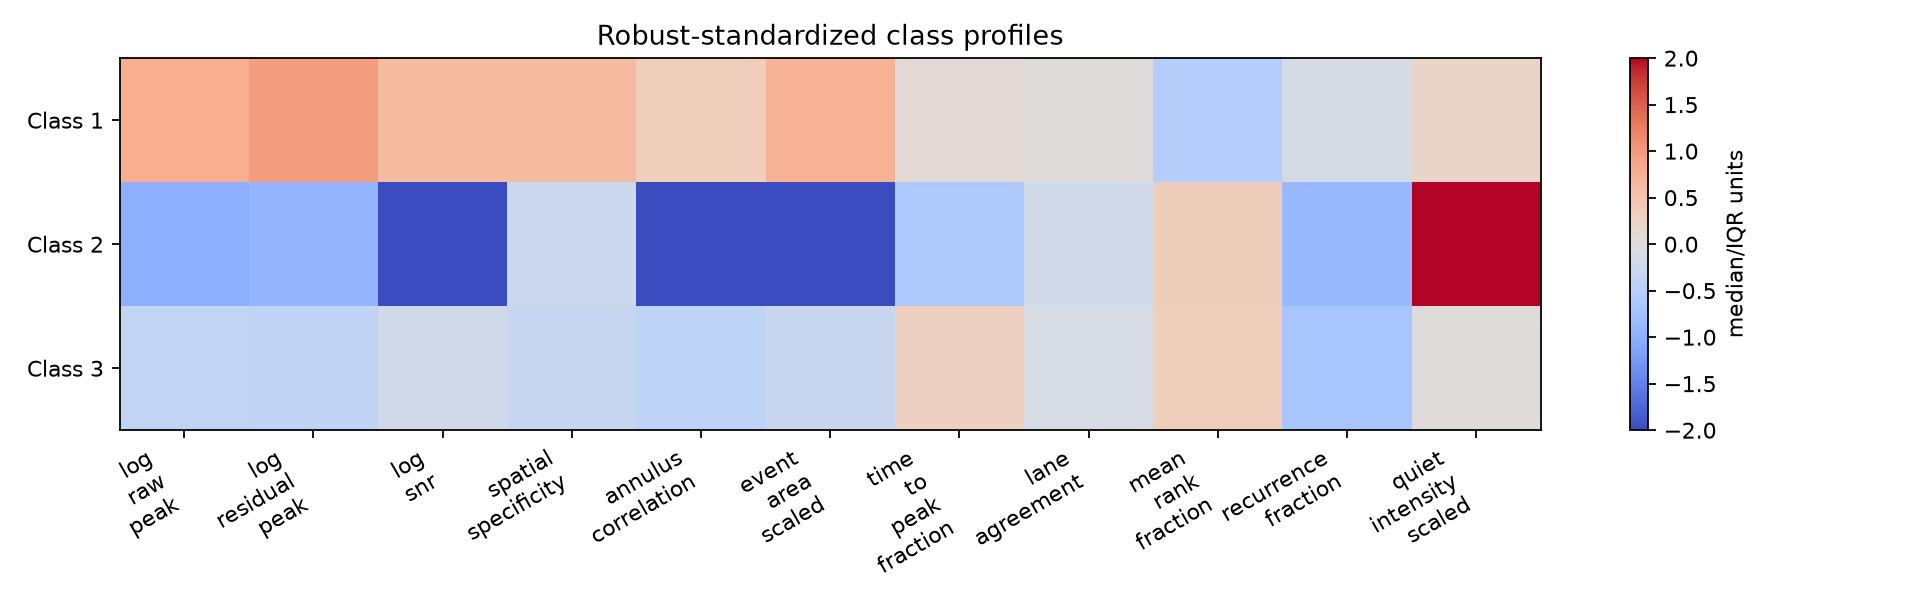
\includegraphics[width=0.98\linewidth]{figures/final/detection_class_profiles.png}
  \caption{Robust-standardized centroids of the three frozen detection-event classes. Signal and contextual measurements were standardized within burst; lane agreement, rank fraction, and recurrence used global robust scaling. Colors show median/IQR units and do not encode expert labels.}
  \label{fig:supp-detection-class-centroids}
\end{figure}

\subsection{Advanced post-freeze class profiling}

\begin{figure}[!htbp]
  \centering
  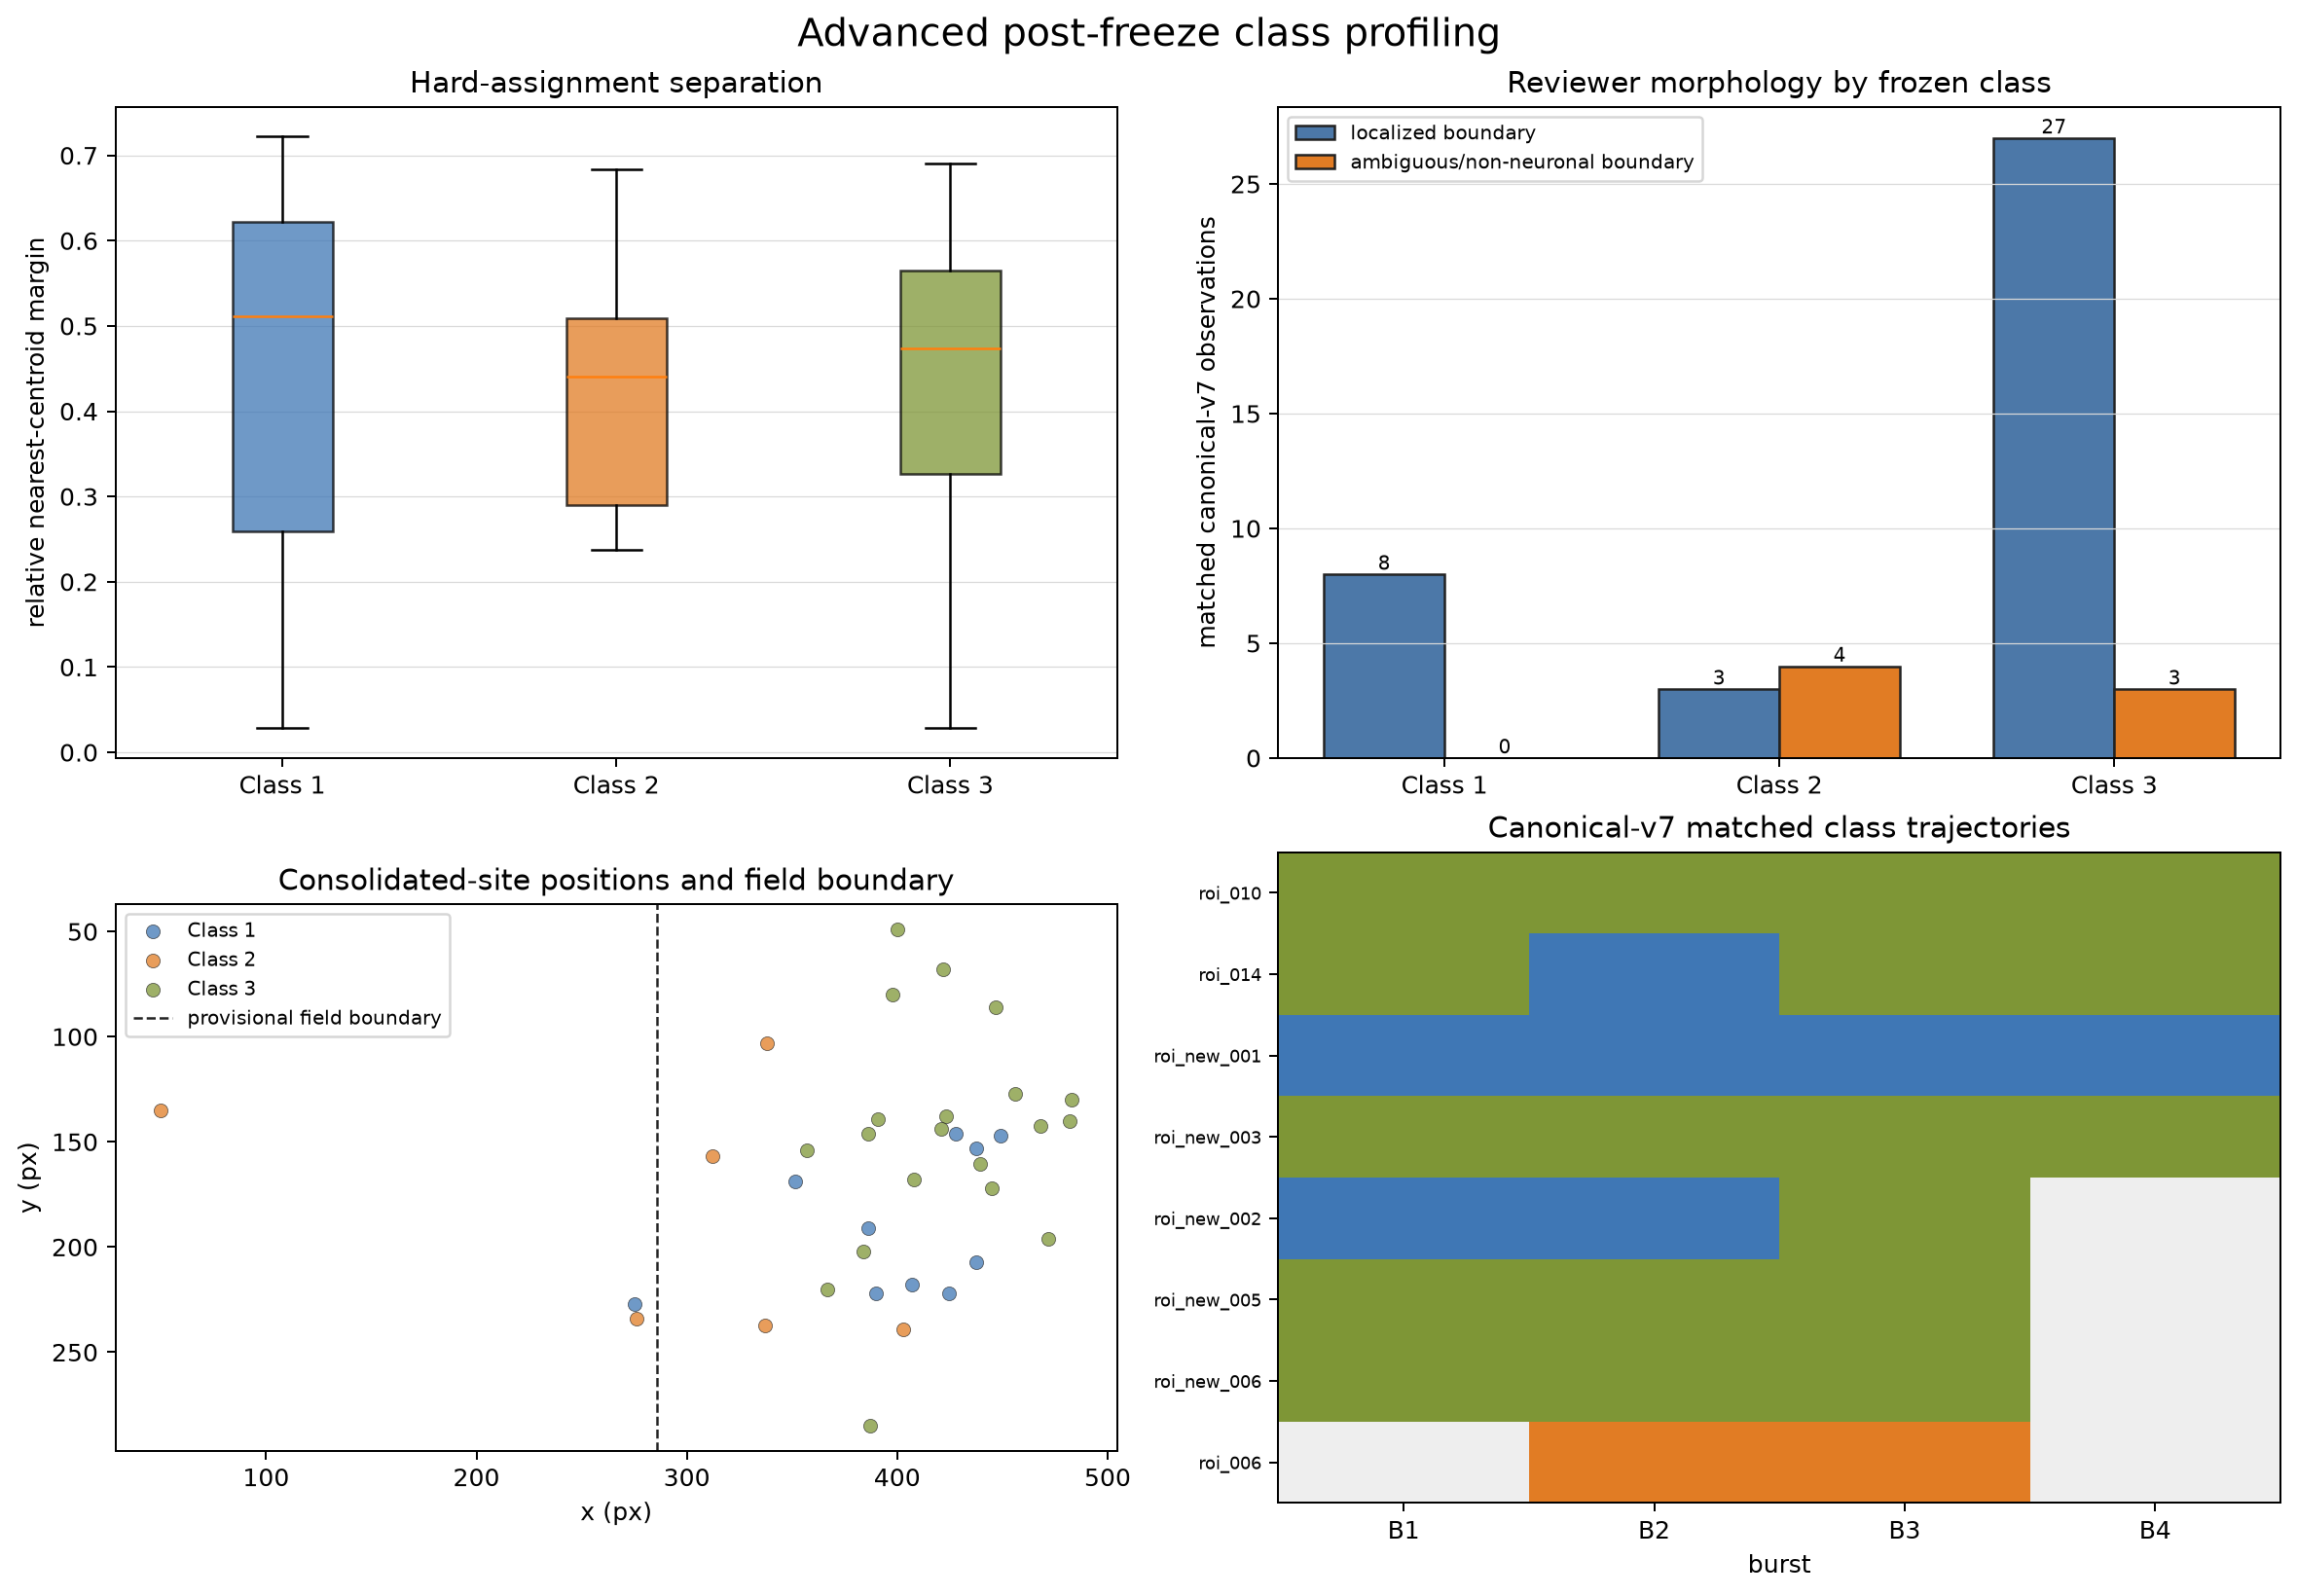
\includegraphics[width=0.98\linewidth]{figures/final/detection_class_advanced_extensions.png}
  \caption{Advanced detection-class extensions. The centroid margin measures relative hard-assignment separation and is not a posterior probability. Reviewer morphology and canonical trajectories use candidate-assisted canonical v7. Spatial positions are consolidated detection sites, so recurrent occurrences do not multiply the field comparison. Gray trajectory cells indicate no matched detection in that burst.}
  \label{fig:supp-detection-class-advanced}
\end{figure}

\subsection{Spatial ICA filter-level stability}

\begin{figure}[!htbp]
  \centering
  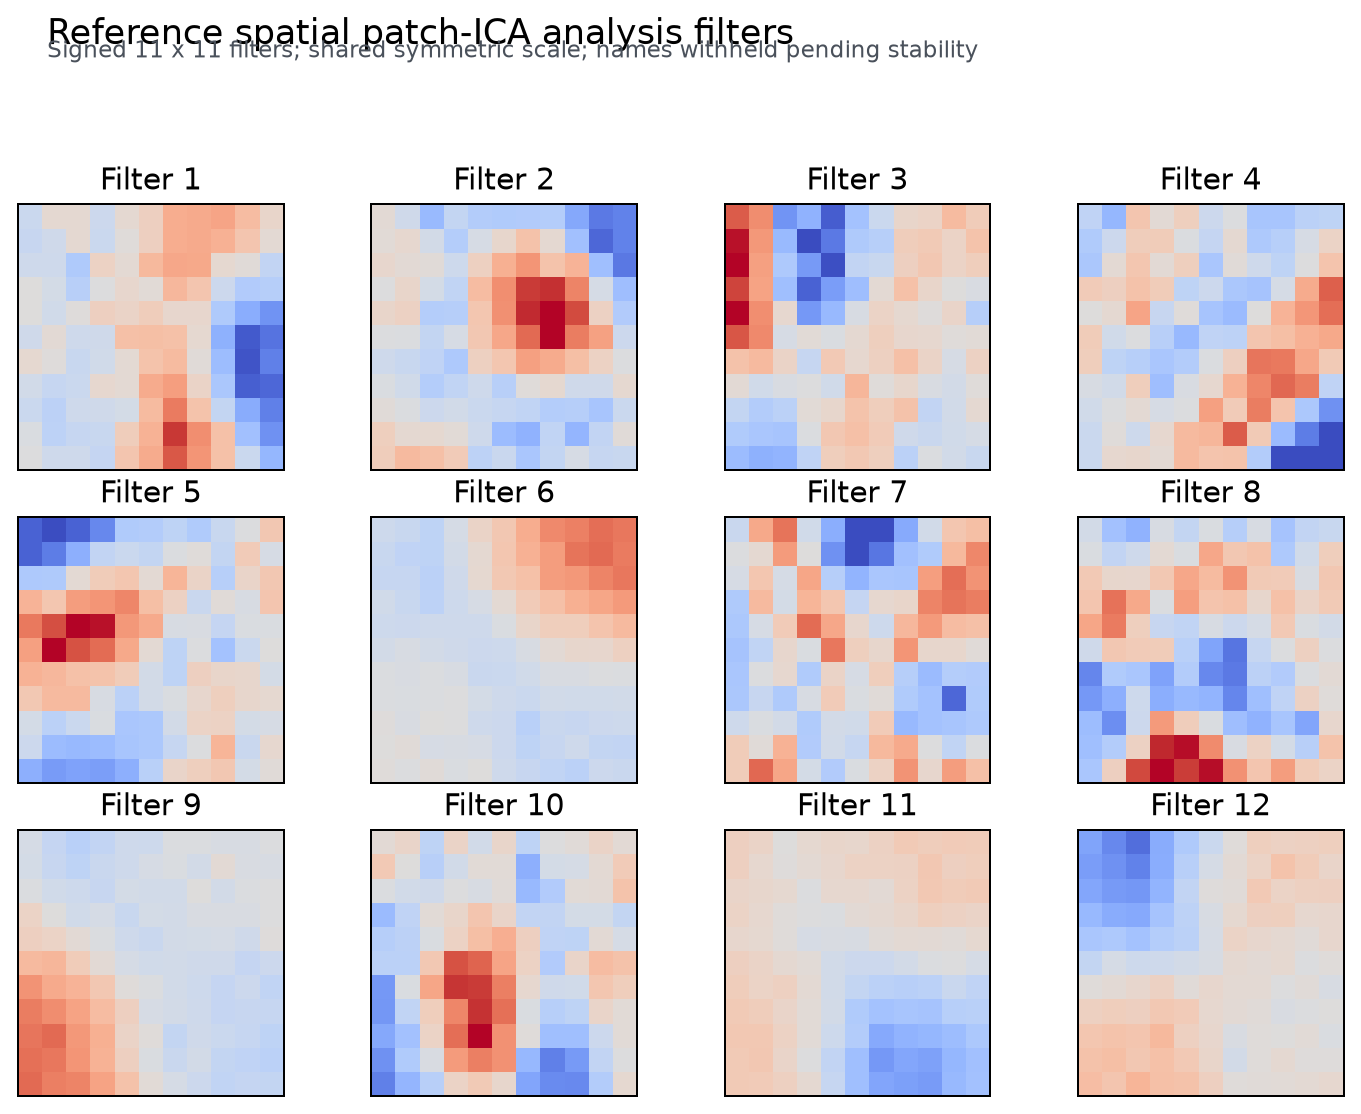
\includegraphics[width=0.98\linewidth]{figures/final/spatial_ica_filter_stability.png}
  \caption{Aligned spatial-ICA filters across random seeds and leave-one-burst-window-out refits. Subspaces were moderately similar, but individual aligned filters failed the prespecified interpretation threshold. The gallery is included to document why component-wise anatomical labels are prohibited even though the reconstructed output is stable.}
  \label{fig:supp-spatial-ica-filter-stability}
\end{figure}

\subsection{Negative and boundary results}

The complete-trace feature panel is an informative boundary result. At
confirmed centers, \FullTraceCarrierCeilingCount{} of \FullTraceOccurrences{}
carrier percentiles and \FullTraceLagCeilingCount{} lagged-recurrence
percentiles equal 1.0. No feature passes the incremental-over-carrier gate.
Consensus and multiscale persistence retain median available burst-pair site-rank
correlations of \FullTraceConsensusRepeatability{} and
\FullTracePersistenceRepeatability{}, but these are exploratory and require
independent-recording transfer. The complete machine-readable feature table is
packaged as \texttt{generated\_analysis/full\_trace\_feature\_panel\_v2/
feature\_summary.tsv}.

The manuscript will preserve scientifically valid negative results. In particular, the final report will state when:
\begin{itemize}
  \item a learned component is analytically equivalent to a simple operator;
  \item a repeatable event waveform is not spatially specific;
  \item a local residual has event amplitude but no stable shape;
  \item a functional or tensor model fails held-out stability;
  \item a representation improves known-positive recovery but materially degrades trace fidelity;
  \item an effect depends on burst~2, one field, one site, or one annotation choice;
  \item precision remains unidentified outside the bounded field.
\end{itemize}
These outcomes constrain future model design and should not be hidden by selective promotion.

\section{Trace-atlas and reviewer-packet specification}
\label{sec:supp-atlas}

\subsection{Per-occurrence atlas page}

Each labeled occurrence receives a stable page keyed by observation identifier. The page contains:
\begin{enumerate}
  \item a full-frame context image with original site, canonical mapping, annulus, outer ring, nearest labeled sites, field boundary, and translated controls;
  \item a high-resolution crop at baseline, proposed onset, Raw peak, residual peak, and event offset;
  \item synchronized native-amplitude traces for Raw, annulus, outer ring, residual, difference, and ICA;
  \item a separate robustly standardized trace panel for shape comparison;
  \item onset, peak, offset, burst interval, saturation, and motion annotations;
  \item a metric card with units and validity flags;
  \item direct links to the source row, mask, trace array, configuration, and generation command.
\end{enumerate}

\DraftFigure{Example layout: context crop at left; full and event-centered traces in the middle; spatial event map, radial profile, and metric/provenance card at right.}{Planned per-occurrence trace-atlas page.}{fig:supp-atlas-page}

\subsection{Per-site summary}

Each immutable site receives a neuron-by-burst summary showing all available occurrences without peak scaling. Required panels are:
\begin{itemize}
  \item Raw and residual traces by burst;
  \item native amplitude and SNR by burst;
  \item spatial event maps and radial profiles;
  \item annulus coupling and specificity;
  \item candidate rank and recovery failure category;
  \item repeatability metrics and uncertainty;
  \item acquisition covariates and field membership;
  \item canonical-identity history and unresolved decisions.
\end{itemize}

\subsection{Reviewer packet}

Review frames are generated independently of detector candidates to avoid circular adjudication. Reviewers receive original-intensity and contrast-normalized views, event movies, the original label, and a standardized response schema. They do not receive representation scores, candidate ranks, or model interpretations. The packet records completion state and supports re-review without changing the immutable source observations.

\subsection{Aggregate atlas index}

The final atlas index supports filtering by burst, original site, proposed canonical identity, field, SNR quantile, morphology, saturation, annulus coupling, timing uncertainty, and recovery status. A machine-readable index mirrors every visual filter and prevents the HTML or PDF atlas from becoming the sole source of truth.


\end{document}
